\chapter{Solutions for Chapter 1}

\ex{1.1}
\begin{enumerate}
    \item 
    $R = \SI{5}{\kohm} + \SI{10}{\kohm} = \mans{\SI{15}{\kohm}}$

    \item 
    $R = \dfrac{R_1 R_2}{R_1 + R_2} = \dfrac{\SI{5}{\kohm} \times \SI{10}{\kohm}}{\SI{5}{\kohm} + \SI{10}{\kohm}} = \mans{\SI{3.33}{\kohm}}$

\end{enumerate}

\ex{1.2}
$P = IV = \left(\dfrac{V}{R}\right)V = \dfrac{(\SI{12}{\V})^2}{\SI{1}{\ohm}} = \mans{\SI{144}{\W}}$

\ex{1.3}
Consider a simple series resistor circuit.
\begin{circuit}{fig:1.3.1}{A basic series circuit.}
    (0,0) to[V=$V$,invert] (0,4)
        to[short,i=$I$] (2,4)
        to[R=$R_1$,v=$V_{1}$] (2,2)
        to[R=$R_2$,v=$V_{2}$] (2,0)
        to (0,0)
\end{circuit}
By KVL and Ohm's law \[ V = V_{1} + V_{2} = R_{1}\cdot I + R_{2} \cdot I = (R_{1}+R_{2}) \cdot I = R \cdot I \]
where \[\mans{R = R_{1} + R_{2}}\] is the resistance of $R_{1}$ and $R_{2}$ in series. Now, consider a simple parallel resistor circuit.

\begin{circuit}{fig:1.3.2}{A basic parallel circuit.}
    (0,0) to[V=$V$,invert] (0,3)
    to[short,i=$I$] (2,3)
    to[R=$R_1$,i>^=$I_{1}$] (2,0);
    \draw (2,3) to[short] (4,3)
    to[R=$R_2$,i>^=$I_{2}$] (4,0)
    to (0,0)
\end{circuit}
By KCL and Ohm's law \[ I = I_{1} + I_{2} = \frac{V}{R_{1}} + \frac{V}{R_{2}} = \left(\frac{1}{R_{1}}+\frac{1}{R_{2}}\right)\cdot V \]
solving for V as a function of I we get
\[V = \dfrac{1}{\frac{1}{R_{1}}+\frac{1}{R_{2}}}\cdot I = \frac{R_{1}R_{2}}{R_{1}+R_{2}}\cdot I = R\cdot I \]
where \[\mans{R = \dfrac{1}{\frac{1}{R_{1}}+\frac{1}{R_{2}}} = \frac{R_{1}R_{2}}{R_{1}+R_{2}}}\] is the resistance of $R_{1}$ and $R_{2}$ in parallel.

\ex{1.4}
We known that the resistance $R_{12}$\footnote{Here we have only assigned a name to the resistance in parallel between $R_{1}$ and $R_{2}$.} of two resistors $R_{1}$ and $R_{2}$ in parallel is given by \[R_{12} = \dfrac{1}{\frac{1}{R_{1}}+\frac{1}{R_{2}}}\]

Now, the resistance $R_{123}$ of three resistors $R_{1}$, $R_{2}$ and $R_{3}$ in parallel is equal to the resistance of two resistors $R_{12}$ (the resistance between $R_{1}$ and $R_{2}$ in parallel) and $R_{3}$ in parallel, then \[R_{123} = \frac{1}{\frac{1}{R_{12}}+\frac{1}{R_{3}}} = \frac{1}{\frac{1}{R_{1}}+\frac{1}{R_{2}}+\frac{1}{R_{3}}}\]

We will prove by induction that the resistance $R_{1\cdots n}$ of $n$ resistances $R_{1}, R_{2}, \ldots, R_{n}$ in parallel is given by \[R_{1\cdots n} = \dfrac{1}{\sum_{i=1}^{n}\frac{1}{R_{i}}}\]

First, it's trivial to show that with $n = 1$ the equality holds. Now, we will assume that the equality is satisfied for $n = k$, that is
\[R_{1\cdots k} = \dfrac{1}{\sum_{i=1}^{k}\frac{1}{R_{i}}}\]

Then, we must show that equality holds for $n = k+1$. Thus, the resistance $R_{1\cdots (k+1)}$ of $(k+1)$ resistances $R_{1}, R_{2}, \ldots, R_{k+1}$ in parallel is equal to the resistance of two resistors $R_{1\cdots k}$ and $R_{k+1}$ in parallel, then \[R_{1\cdots (k+1)} = \frac{1}{\frac{1}{R_{1\cdots k}}+\frac{1}{R_{k+1}}} = \frac{1}{\sum_{i=1}^{k}\frac{1}{R_{i}}+\frac{1}{R_{k+1}}} = \frac{1}{\sum_{i=1}^{k+1}\frac{1}{R_{i}}}\]
where we have proved that equality holds for $n = k+1$. Finally, the resistance of $n$ resistors in parallel is given by \[\mans{R_{1\cdots n} = \dfrac{1}{\sum_{i=1}^{n}\frac{1}{R_{i}}} = \frac{1}{\frac{1}{R_{1}}+\frac{1}{R_{2}}+\ldots+\frac{1}{R_{n}}}}\]

\ex{1.5}
Given that $P = \dfrac{V^2}{R}$, we know that the maximum voltage we can achieve is \SI{15}{\V} and the smallest resistance we can have across the resistor in question is \SI{1}{\kohm}. Therefore, the maximum amount of power dissipated can be given by \[P = \frac{V^2}{R} = \frac{(\SI{15}{\V})^2}{\SI{1}{\kohm}} = \mans{\SI{0.225}{\W}}\]
This is less than the \SI{0.25}{\W} power rating.

\ex{1.6}
\begin{enumerate}
    \item
    The total current required by New York City that will flow through the
    cable is 
    \[I = \frac{P}{V} = \frac{\SI{1e10}{\W}}{\SI{115}{\V}} = \SI{86.96}{\mega\A}\]
    Therefore, the total power lost per foot of cable can be calculated by:
    \[P = I^2R = \left(\SI{86.96e6}{\A}\right)^2 \times \left(\SI{5e-8}{\ohm\per ft}\right) = \mans{\SI{3.78e8}{\W\per ft}}\] 
    \item
    The length of cable over which all $\SI{1e10}{\W}$ will be lost is:
    \[L = \frac{\SI{1e10}{\W}}{\SI{3.78e8}{\W\per ft}} = \mans{\SI{26.45}{ft}}\]
    \item
    To calculate the heat dissipated by the cable, we can use the Stefan-Boltzmann equation $T = \sqrt[4]{\frac{P}{A\sigma}}$, with A corresponding to the cylindrical surface area of the \SI{26.45}{ft} section of 1-foot diameter cable. Note that $\sigma$ is given in \si{\cm^2}, so we will need to use consistent units.
    \[A = \pi DL = \pi \times \SI{30.48}{\cm}\times \SI{806.196}{\cm} = \SI{7.72e4}{\cm^2}\]
    Therefore,
    \[T = \sqrt[4]{\frac{P}{A\sigma}} = \sqrt[4]{\frac{\SI{1e10}{\W}}{\SI{7.72e4}{\cm^2} \times \SI{6e-12}{\W\per\kelvin^4\per\cm^2}}} = \mans{\SI{12121}{K}} \]
    This is indeed a preposterous temperature, more than twice that at the surface of the Sun! The solution to this problem is that power should be transmitted along long distances at high voltage. This greatly reduces $I^2R$ losses. For example, a typical high voltage line voltage is $\SI{115}{\kV}$. At this voltage, the power loss per foot of cable is only \SI{378}{\W} per foot. Intuitively, we know that reducing current allows for lower power dissipation. We can deliver the same amount of power with a lower current by using a higher voltage.
\end{enumerate}

\ex{1.7}
A \SI{20000}{\ohm\per\V} meter read, on its \SI{1}{\V} scale, puts a $\SI{20000}{\ohm\per\V} \cdot \SI{1}{\V} = \SI{20000}{\ohm} = \SI{20}{\kohm}$ resistor in series with an ideal ammeter (ampere meter). Also, a voltage source with an internal resistance is equivalent to an ideal voltage source with its internal resistance in series.
\begin{enumerate}
    \item In the first question, we have the following circuit:
    \begin{circuit}{fig:1.7.1}{A voltage source with internal resistance and a \SI{20000}{\ohm\per\V} meter read in its \SI{1}{\V} scale.}
        (0,0) to[V=\SI{1}{\V},invert] (0,4)
        to[R=\SI{10}{\kohm},i>^=$I$] (5,4);
        \draw[blue] (5,4) to[R=\SI{20}{\kohm},*-,color=blue] (5,2)
        to node[draw,circle,fill=white] {A} (5,0);
        \draw[blue] node[draw,circle,fill=blue,inner sep=1pt] at(5,0) {};
        \draw (5,0) to (0,0)
    \end{circuit}
    Then, we have that the current in the ideal ammeter and the voltage in the meter resistance are given by\footnote{When a meter only measures currents, it puts a resistance in series to measures the current through that resistance and internally converts that current into voltage to \textit{measure voltages}.}
    \[I = \frac{\SI{1}{\V}}{\SI{10}{\kohm} + \SI{20}{\kohm}} = \mans{\SI{0.0333}{\mA}} \quad \text{ and } \quad V = \SI{0.0333}{\mA} \times \SI{20}{\kohm} = \mans{\SI{0.666}{\V}}\]
    \item In the second question, we have the following circuit:
    \begin{circuit}{fig:1.7.2}{A $\SI{10}{\kohm}-\SI{10}{\kohm}$ voltage divider and a $\SI{20000}{\ohm\per\V}$ meter read in its $\SI{1}{\V}$ scale.}
        (0,0) to[V=$\SI{1}{\V}$,invert] (0,4)
        to[short] (3,4)
        to[R=$\SI{10}{\kohm}$] (3,2)
        to[R=$\SI{10}{\kohm}$] (3,0);
        \draw[blue] (3,2) to node[draw,circle,fill=white] {A} (5,2)
        to[R=$\SI{20}{\kohm}$,color=blue] (5,0)
        to[short,-*,color=blue] (3,0);
        \draw[blue] node[draw,circle,fill=blue,inner sep=1pt] at(3,2) {};
        \draw (3,0) to (0,0)
    \end{circuit}
    Now, we can to obtain the Thévenin equivalent circuit of circuit in Figure \ref{fig:1.7.2} with
    \[R_{\Th} = \frac{\SI{10}{\kohm} \cdot \SI{10}{\kohm}}{\SI{10}{\kohm} + \SI{10}{\kohm}} = \SI{5}{\kohm}\]
    and
    \[V_{\Th} = \SI{1}{\V} \cdot \frac{\SI{10}{\kohm}}{\SI{10}{\kohm} + \SI{10}{\kohm}} = \SI{0.5}{\V}\]
    Then, we have the following equivalent circuit:
    \begin{circuit}{fig:1.7.3}{Thévenin equivalent circuit of circuit in Figure \ref{fig:1.7.2}.}
        (0,0) to[V=$V_{\Th}$,invert] (0,4)
        to[R=$R_{\Th}$,i>^=$I$] (5,4);
        \draw node[draw,circle,fill=blue,inner sep=1pt] at(5,4) {};
        \draw[blue] (5,4)
        to node[draw,circle,fill=white] {A} (5,2)
        to[R=$\SI{20}{\kohm}$,-*,color=blue] (5,0);
        \draw (5,0) to (0,0)
    \end{circuit}
    Finally, we have that the current in the ideal ammeter and the voltage in the meter resistance are given by
    \[I = \frac{\SI{0.5}{\V}}{\SI{5}{\kohm} + \SI{20}{\kohm}} = \mans{\SI{0.02}{\mA}} \quad \text{ and } \quad V = \SI{0.02}{\mA} \cdot \SI{20}{\kohm} = \mans{\SI{0.4}{\V}}\]
\end{enumerate}

\ex{1.8}
\begin{enumerate}
    \item In the first part, we have the following circuit:
    \begin{circuit}{fig:1.8.1}{\SI{50}{\uA} ammeter with \SI{5}{\kohm} internal
        resistance (shown in blue) in parallel with shunt resistor.}

        (0,0) to[isource, l=$I$, -*] (0,2)
        (0,2) to[short] (0,3);
        \draw[blue]
        (0,2) to[R=\SI{5}{\kohm}, i>^=$I_m$, color=blue] (4,2)
        (4,2) to node[draw, circle, fill=white] {A} (6,2);
        \draw
        (0,3) to[R=$R_s$, i>^=$I_s$] (6,3)
        (6,3) to[short, -*] (6,2)
        (6,2) to[short] (6,0)
        (6,0) to[short] (0,0)
    \end{circuit}

    We want to measure $I$ for 0-1 A, and the ideal ammeter measures
    up to \SI{50}{\uA}. To find what shunt resistance $R_s$ allows us to do so,
    we set $I = \SI{1}{\A}$ and $I_m = \SI{50}{\uA}$. By KCL we know $I_s = \SI{0.999950}{\A}$.
    To determine $R_s$, we still need to find the voltage across it. We can
    find this voltage by doing
    \[V = I_m R_m = \SI{50}{\uA} \cdot \SI{5}{\kohm} = \SI{0.25}{\V}\]
    Then we simply do
    \[R_s = \frac{V}{I_s} = \frac{\SI{0.25}{\V}}{\SI{0.999950}{\A}} = \mans{\SI{0.25}{\ohm}}\]

    \item In the second part, we have the following circuit:
    \begin{circuit}{fig:1.8.2}{\SI{50}{\uA} ammeter with \SI{5}{\kohm} internal
        resistance (shown in blue) with a series resistor.}

        (0,0) to[V=$V$, invert, i^>=$I$] (0,2);
        \draw[blue]
        (0,2) to[R=\SI{5}{\kohm}, color=blue] (2,2)
        (2,2) to node[draw, circle, fill=white] {A} (4,2);
        \draw
        (4,2) to[R=$R_s$] (4,0)
        (4,0) to[short] (0,0)
    \end{circuit}
    We want to measure $V$ for 0-10 V, and the ideal ammeter measures up to
    \SI{50}{\uA}. To find the series resistance $R_s$, we set $V = \SI{10}{\V}$ and
    $I = \SI{50}{\uA}$. Then we solve
    \[\frac{V}{I} = \SI{5}{\kohm} + R_s\]
    \[R_s = \frac{\SI{10}{\V}}{\SI{50}{\uA}} - \SI{5}{\kohm} = \mans{\SI{195}{\kohm}}\]
\end{enumerate}

\ex{1.9}
In order to measure resistance well above the range of your multimeter, you need to get creative.  We will be using the multimeter in voltmeter mode.  Lets start by connecting our DC voltage source, voltmeter, and the high-value resistor in series.  (The reason for doing this will become clear later).

\begin{circuit}{fig:1.9.1}{Connection of three components.}
    (0,2) to[V=$V_{\in}$] (0,0)
    (0,2) to[qvprobe=voltmeter] (4,2)
    (4,2) to[R=$R_L$] (4,0)
    (4,0) to[short] (0,0)
\end{circuit}

$V_{\in}$ is our test voltage, and $R_L$ is our leakage resistance. We need to revise the model for our voltmeter.

\begin{circuit}{fig:1.9.2}{The voltmeter is now modeled as a resistor with value $R_M$.}
    (0,2) to[V=$V_{\in}$] (0,0)
    (0,2) to[short, i>^=$I_{\in}$] (1,2)
    (1,2) to[R=$R_M$, i>_=$I_M$] (3,2)
    (3,2) to[short] (4,2)
    (4,2) to[R=$R_L$, i>_=$I_L$] (4,0)
    (4,0) to[short] (0,0)
\end{circuit}

The current flowing through our meter (modeled by the resistor $R_M$) is equal to the current flowing through the leakage resistor. This is also equal to the current supplied from our voltage source.
\[I_M = I_L = I_{\in}\]

\begin{circuit}{fig:1.9.3}{Voltage and current labels are added.}
    (0,2) to[V=$V_{\in}$] (0,0)
    (0,2) to[short, i>^=$I_{\in}$] (1,2)
    (1,2) to[R=$R_M$, v_>=$V_M$] (3,2)
    (3,2) to[short] (4,2)
    (4,2) to[R=$R_L$, v_>=$V_L$] (4,0)
    (4,0) to[short] (0,0)
\end{circuit}

Notice: this test circuit is a \textbf{voltage divider}.  When you use this technique, the voltmeter itself makes up half of the divider. The voltage across the leakage resistor cannot be measured directly, so we calculate it using Kirchhoff's Voltage Law by subtracting our voltmeter's reading from the voltage of our DC supply.
\[V_L = V_{\in} - V_M\]
The current through the voltmeter's resistance is given by Ohm's Law.
\[I_M = \frac{V_M}{R_M}\]
The current through the leakage resistor is given by Ohm's Law.
\[I_L = \frac{V_L}{R_L}\]
We already determined that $I_M$ and $I_L$ are equal, so we can set the two previous expressions equal to each other.
\[I_M = I_L  \Rightarrow  \frac{V_M}{R_M} = \frac{V_L}{R_L}\]
We will rearrange the above equation to give an expression for $R_L$.
\[R_L = R_M \frac{V_L}{V_M}\]
Now we can substitute our first expression for $V_L$ into the previous equation to eliminate $V_M$ (the final unknown term).
\[R_L = R_M \frac{V_{\in} - V_M}{V_M}\]
Rewriting the equation, the final result is
\[\mans{R_L = R_M \left(\frac{V_{\in}}{V_M} - 1\right)}\]

To measure leakage current with a voltmeter, simply divide the meter's reading by the resistance of the meter.  For example, if your \SI{10}{\Mohm} voltmeter measures \SI{0.023}{\V}, then $I_{leakage} = \SI{23}{\mV} / \SI{10}{\Mohm} = \SI{2.3}{\nA}$.  The accuracy of such a measurement depends both on the accuracy of the voltage measurement, and the tolerance of the meter's resistance.

\ex{1.10}
\begin{enumerate}
    \item 
    With two equal-value resistors, the output voltage is half the input voltage.
    \[V_\out = \frac{1}{2}V_\in = \frac{\SI{30}{\V}}{2} = \mans{\SI{15}{\V}}\]

    \item 
    To treat $R_2$ and $R_{\load}$ as a single resistor, combine the two resistors which are in parallel to find that the combined (equivalent) resistance is \SI{5}{\kohm}. Now, we have a simple voltage divider with a \SI{10}{\kohm} resistor in series with the \SI{5}{\kohm} equivalent resistor. The output voltage is across this equivalent resistance. The output voltage is given by 
    \[V_\out = V_{\in} \frac{\SI{5}{\kohm}}{\SI{10}{\kohm} + \SI{5}{\kohm}} = \frac{\SI{30}{\V}}{3} = \mans{\SI{10}{\V}} \]
    \begin{circuit}{fig:1.10.1}{Voltage divider with simplified equivalent resistance}
        % \label{1.10fig1}
        (0,2) to[V=$V_{\in}$] (0,0)
        to[short] (2,0)
        to[R=$R_{eq}$] (2,2)
        to[R=$R_1$](0,2)
        (2,0) to[short, *-o] (3,0)
        (2,2) to[short, *-o] (3,2)
        (3,0) to[open, v_<=$V_\out$] (3,2)
    \end{circuit}

    \item 
    We can redraw the voltage divider circuit to make the ``port'' clearer. 
    \begin{circuit}{fig:1.10.2}{Voltage divider with port shown.}
        % \label{1.10fig1}
        (0,2) to[V=$V_\in$] (0,0)
        to[short] (2,0)
        to[R=$R_2$] (2,2)
        to[R=$R_1$](0,2)
        (2,0) to[short, *-o] (3,0)
        (2,2) to[short, *-o] (3,2)
        (3,0) to[open, v_<=$V_\out$] (3,2)
    \end{circuit}

    We can find $V_\Th$ by leaving the ports open (open circuit) and measuring $V_\out$, the voltage across $R_2$. This comes out to be half the input voltage when $R_1 = R_2$, so $V_\out = \SI{15}{\V}$. Thus $V_{\Th} = \mans{\SI{15}{\V}}$.
    
    To find the Th\'evinen resistance, we need to find the short circuit current, $I_{SC}$. We short circuit the port and measure the current flowing through it.
    \begin{circuit}{fig:1.10.3}{Voltage divider with short circuit on the output.}
        (0,2) to[V=$V_\in$] (0,0) 
        to[short] (2,0)
        to[R=$R_2$] (2,2)
        to[R=$R_1$](0,2)
        (2,0) to[short] (3,0)
        (2,2) to[short] (3,2)
        (3,0) to[short, i_<=$I_{SC}$] (3,2) 
    \end{circuit}
    
    In this circuit, no current flows through $R_2$, flowing through the short instead. Thus we have $I_{SC} = \dfrac{V_\in }{R_1}$. From this, we can find $R_\Th$ from $R_\Th = \dfrac{V_\Th}{I_{SC}}$. This gives us 
    \[R_\Th = \frac{V_\Th}{I_{SC}} = \frac{V_\Th}{V_\in/R_1} = \frac{\SI{15}{\V}}{\SI{30}{\V}/\SI{10}{\kohm}} = \mans{\SI{5}{\kohm}}\]

    The Th\'evenin equivalent circuit takes the form shown below.
    \begin{circuit}{fig:1.10.4}{Th\'evenin equivalent circuit.}
        (0,2) to[V=$V_\Th$] (0,0)
        to[short, -o] (3,0)
        (0,2) to[R=$R_\Th$, -o] (3,2)
        (3,0) to[open, v_<=$V_\out$] (3,2)
    \end{circuit}
    In terms of behavior at the ports, this circuit is equivalent to the circuit in Figure \ref{fig:1.10.1}. 

    \item 
    We connect the $\SI{10}{\kohm}$ load to the port of the Th\'evenin equivalent circuit in Figure \ref{fig:1.10.4} to get the following circuit.
    \begin{circuit}{fig:1.10.5}{Th\'evenin equivalent circuit with $\SI{10}{\kohm}$ load.}
        (0,2) to[V=$V_{\Th}$] (0,0)
        to[short] (3,0)
        (0,2) to[R=$R_{\Th}$] (3,2)
        (3,0) to[R=$\SI{10}{\kohm}$, v_<=$V_\out$] (3,2)
    \end{circuit}
    From here, we can find $V_\out$, treating this circuit as a voltage divider.
    \[V_\out = \frac{\SI{10}{\kohm}}{R_\Th + \SI{10}{\kohm}} V_\Th = \frac{\SI{10}{\kohm}}{\SI{5}{\kohm} + \SI{10}{\kohm}} \cdot \SI{15}{\V} = \mans{\SI{10}{\V}}\] 
    This is the same answer we got in part (b).

    \item 
    To find the power dissipated in each resistor, we return to the original three-resistor circuit. 
    \begin{circuit}{fig:1.10.6}{Original voltage divider with $\SI{10}{\kohm}$ load attached.}
        (0,2) to[V, l_=$V_\in$] (0,0)
            to[short] (3,0)
            to[R, l_=$R_\load$] (3,2)
            to[short] (2,2)
            to[R=$R_1$] (0,2)
        (2,0) to[R=$R_2$, *-*] (2,2)
    \end{circuit}

    From part (d), we know that the output voltage is 10V and that this is the voltage across the load resistor. Since $P = IV = \frac{V^2}{R}$, we find that the power through $R_\load$ is 
    \[P_\load = \frac{V^2}{R_\load} = \frac{(\SI{10}{\V})^2}{\SI{10}{\kohm}} = \mans{\SI{10}{\mW}}\]
    Similarly, we know that the power across $R_2$ is the same since the voltage across $R_2$ is the same as the voltage across $R_\load$. Thus we have
    \[P_2 = \mans{\SI{10}{\mW}}\]
    To find the power dissipated in $R_1$, we first have to find the voltage across it. From Kirchoff's loop rule, we know that the voltage around any closed loop in the circuit must be zero. We can choose the loop going through the voltage source, $R_1$, and $R_2$. The voltage supplied by the source is 30V. The voltage dropped across $R_2$ is 10V as discussed before. Thus the voltage dropped across $R_1$ must be $\SI{30}{\V} - \SI{10}{\V} - \SI{20}{\V}$. Now we know the voltage across and the resistance of $R_1$. We use the same formula as before to find the power dissipated.
    \[P_1 = \frac{V^2}{R_1} = \frac{(\SI{20}{\V})^2}{\SI{10}{\kohm}} = \mans{\SI{40}{\mW}}\]
\end{enumerate}

\ex{1.11}
Consider the following Th\'evenin circuit where $R_\source$ is just another name for the Th\'evenin resistance, $R_\Th$.
\begin{circuit}{fig:1.11.1}{Standard Th\'evenin circuit with attached load.}
    (0,2) to[V, l_=$V_\Th$] (0,0)
        to[short] (2,0)
        to[R, l_=$R_\load$] (2,2)
        to[R, l_=$R_\source$] (0,2)
\end{circuit}
We will first calculate the power dissipated in the load and then maximize it with calculus. We can find the power through a resistor using current and resistence since $P = IV = I(IR) = I^2R$. To find the total current flowing through the resistors, we find the equivalent resistance which is $R_\source + R_\load$. Thus the total current flowing is $I = \dfrac{V_\Th}{R_\source + R_\load}$. The power dissipated in $R_\load$ is thus 
\[P_\load = I^2R_\load = \dfrac{V_\Th^2 R_\load}{(R_\source + R_\load)^2}\]
To maximize this function, we take the derivative and set it equal to 0.
\begin{align*}
    \frac{dP_\load}{dR_\load} &= V_\Th \frac{(R_\source + R_\load)^2 - 2R_\load(R_\source + R_\load)}{(R_\source + R_\load)^4} = 0 \\
    &\Longrightarrow R_\source + R_\load = 2R_\load \\
    &\Longrightarrow R_\source = R_\load
\end{align*}

\ex{1.12}
\begin{enumerate}
    \item 
    Voltage ratio: $\frac{V_2}{V_1} = 10^{\si{\dB}/20} = 10^{3/20} = \mans{1.413}$

    Power ratio: $\frac{P_2}{P_1} = 10^{\si{\dB}/10} = 10^{3/10} = \mans{1.995}$

    \item 
    Voltage ratio: $\frac{V_2}{V_1} = 10^{\si{\dB}/20} = 10^{6/20} = \mans{1.995}$

    Power ratio: $\frac{P_2}{P_1} = 10^{\si{\dB}/10} = 10^{6/10} = \mans{3.981}$
    
    \item 
    Voltage ratio: $\frac{V_2}{V_1} = 10^{\si{\dB}/20} = 10^{10/20} = \mans{3.162}$

    Power ratio: $\frac{P_2}{P_1} = 10^{\si{\dB}/10} = 10^{10/10} = \mans{10}$
    
    \item 
    Voltage ratio: $\frac{V_2}{V_1} = 10^{\si{\dB}/20} = 10^{20/20} = \mans{10}$

    Power ratio: $\frac{P_2}{P_1} = 10^{\si{\dB}/10} = 10^{20/10} = \mans{100}$
\end{enumerate}

\ex{1.13}
There are two important facts to notice from Exericse 1.12:
\begin{enumerate}[label=\arabic*.]
    \item 
    An increase of \SI{3}{\dB} corresponds to doubling the power 
    
    \item 
    An increase of \SI{10}{\dB} corresponds to 10 times the power.
\end{enumerate}
Using these two facts, we can fill in the table. Start from \SI{10}{\dB}. Fill in \SI{7}{\dB}, \SI{4}{\dB}, and \SI{1}{\dB} using fact 1. Then fill in \SI{11}{\dB} using fact 2. Then fill in \SI{8}{\dB}, \SI{5}{\dB}, and \SI{2}{\dB} using fact 1 and approximating 3.125 as $\pi$.

\begin{center}
    \begin{tabular}{c|c}
        \si{\dB} & ratio($P/P_0$) \\ \hline 
        0 & 1\\
        1 & \tans{1.25}\\
        2 & $\mans{\pi/2}$\\
        3 & 2\\
        4 & \tans{2.5}\\
        5 & \tans{3.125 $\approx \pi$}\\
        6 & 4\\
        7 & \tans{5}\\
        8 & \tans{6.25}\\
        9 & 8\\
        10 & 10\\
        11 & \tans{12.5}
    \end{tabular}
\end{center}

\ex{1.14}
Recall the relationship between $I$, $V$, and $C$: $I = C\frac{dV}{dt}$. Now, we perform the integration:
\begin{align*}
    \int dU &= \int_{t_0} ^{t_1} VIdt\\
    U &= \int_{t_0} ^{t_1} CV\frac{dV}{dt}dt\\
    &= C\int_0^{V_f} V dV\\
    U &= \frac{1}{2}CV_f^2
\end{align*}

\ex{1.15}
Consider the following two capacitors in series.
\begin{circuit}{fig:1.15.1}{Two capacitors in series.}
    (0,0) to[C=$C_1$] (2,0)
        to[C=$C_2$] (4,0)
    (-0.5,-0.5) to[open, v_>=$V_\text{total}$] (4.5,-0.5)
\end{circuit}

To prove the capacitance formula, we need to express the total capacitance of both of these capacitors in terms of the individual capacitances. From the definition of capacitance, we have 
\[C_\text{total} = \frac{Q_\text{total}}{V_\text{total}}\]
Notice that $V_\text{total}$ is the sum of the voltages across $C_1$ and $C_2$. We can get each of these voltages using the definition of capacitance.
\[V_\text{total} = V_1 + V_2 = \frac{Q_1}{C_1} + \frac{Q_2}{C_2}\]
The key observation now is that because the right plate of $C_1$ is connected to the left plate of $C_2$, the charge stored on both plates must be of equal magnitude.\footnotemark Therefore, we have $Q_1 = Q_2$. Let us call this charge stored $Q$ (i.e. $Q = Q_1 = Q_2$). Now, we know that the total charge stored is also $Q$.\footnotemark Therefore, we know that $Q_\text{total} = Q$. Now, we have 
\[C_\text{total} = \frac{Q_\text{total}}{V_\text{total}} = \frac{Q}{Q_1/C_1 + Q_2/C_2} = \frac{Q}{Q/C_1 + Q/C_2} = \frac{1}{1/C_1 + 1/C_2}\]

\footnotetext{If this were not true, then there would be a net charge on these two plates and the wire between them. Because we assume that the capacitors started out with no net charge and there is no way for charge to leave the middle wire or the two plates it connects, this is impossible. }

\footnotetext{If you are having trouble seeing this, suppose we apply a positive voltage to the left plate of $C_1$ relative to the right plate of $C_2$. Suppose this causes the left plate of $C_1$ to charge to some charge $q$. We now must have a charge of $-q$ on the right plate of $C_1$ because $q$ units of charge are now pushed onto the left plate of $C_2$. Now the left of $C_2$ has $q$ units of charge which causes a corresponding $-q$ charge on the right side of $C_2$. Thus the overall total charge separated across these two capacitors is $q$. 
}

\ex{1.16}
Equation 1.21 gives us the relationship between the time and the voltage ($V_\out$) across the capacitor while charging. To find the rise time, subtract the time it takes to reach 10\% of the final value from the time it takes to reach 90\% of the final value.
\begin{align*}
    V_\out &= 0.1V_f = V_f(1-e^{-t_1/RC}) \\
    0.1 &= 1 - e^{-t_1/RC}\\ 
    t_1 &= -RC \ln(0.9)
\end{align*}
Similarly, we find that $t_2 = -RC \ln(0.1)$. Subtracting these two gives us 
\[t_2 - t_1 = -RC(\ln(0.1) - \ln(0.9)) = 2.2RC\]

\ex{1.17}
The voltage divider on the left side of the circuit can be replaced with the Th\'evenin equivalent circuit found Exercise 1.10 (c). Recall that $V_\Th = \frac{1}{2} V_\in$ and $R_\Th = \SI{5}{\kohm}$. This gives us the following circuit.
\begin{circuit}{fig:1.17.1}{Th\'evenin equivalent circuit to Figure 1.36 from the textbook.}
    (0,2) to[open, v_>=$V_\Th$, o-o] (0,0) node[ground]{}
    (0,2) to[R=$R_\Th$] (3,2)
        to[C=$C$, *-] (3,0) node[ground]{}
    (3,2) to[short, -o] (5,2)
    to[open, v^>=$V(t)$, o-o] (5,0) node[ground]{}
\end{circuit}

Now we have a simple RC circuit which we can apply Equation 1.21 to. The voltage across the capacitor is given by 
\[V(t) = V_\text{final}(1 - e^{-t/RC}) = V_\Th (1 - e^{-t/R_\Th C} = \mans{\frac{1}{2}V_\in (1 - e^{-t/5 \times 10^{-4}})}\]

\begin{plot}{fig:1.17.2}{V(t) sketch.}
    [->] (0,0) -- (6,0) node[right] {$t /ms$};
    \draw[->] (0,0) -- (0,5) node[left] {$V$};
    \draw[smooth, domain = 0:6, color=black, thick] plot (\x,{1/2*8*(1-e^(-\x/0.5))});
    \fill [blue] ($(0,0)$) circle (1.5pt) node at (1.4,0)[left] {\color{blue}$(0,0)$};
    \node at (4.5,4.5)[right] {\footnotesize\color{blue}$\frac{1}{2}V_\in (1 - e^{-t/(5 \times 10^{-4})})$};
    \draw[smooth, dashed, domain=0:4.5, color=gray] plot (\x,4);
    \node at (0,4)[left] {\footnotesize\color{blue}$\frac{1}{2}V_\in$};
    \fill [blue] ($(0.5,2.52)$) circle (1.5pt) node at (0.5,2.5)[right] {\color{blue}$(0.5,\frac{1}{2}V_\in \times 63\%)$};
\end{plot}

\ex{1.18}
From the capacitor equation in the previous paragraph, we have 
\[V(t) = (I/C)t = (\SI{1}{\mA}/\SI{1}{\micro\farad}) \times t = \SI{10}{\V}\]
This gives us
\[\mans{t = \SI{0.01}{\s}}\]

\ex{1.19}
Suppose a current \(I\) is flowing through a loop of wire with cross-sectional area \(A\).
This induces a magnetic field \(B\), and the flux \(\Phi\) through the loop is
\[\Phi = BA\]
Now suppose the same current \(I\) flows through a wire coiled into \(n\) loops, each with the same cross-sectional area \(A\).
This induces a magnetic field of \(n\) times the strength, \(B_n = nB\). Since each loop has area \(A\),
the total cross-sectional area of the coil can be considered \(A_n = nA\). Then the magnetic flux
through the coil is
\[\Phi_n = B_nA_n = n^2BA = n^2\Phi\]
Since inductance is defined as flux through a coil divided by current through the flux,
we can see that \(\Phi_n = n^2\Phi\) implies \(L \propto n^2\).

\ex{1.20}
We can use the formula for the full-wave rectifier ripple voltage to find the capacitance.
\[\frac{I_\load}{2fC} = \Delta V \le 0.1 \text{V}_\pp\]
The maximum load current is 10mA and assuming a standard wall outlet frequency of 60 Hz, we have
\[C \ge \frac{\SI{10}{\mA}}{2\times \SI{60}{\Hz} \times \SI{0.1}{\V}} = \mans{\SI{833}{\micro\farad}}\]
Now we need to find the AC input voltage. The peak voltage after rectification must be \SI{10}{\V} (per the requirements). Since each phase of the AC signal must pass through 2 diode drops, we have to add this to find out what our AC peak-to-peak voltage must be. Thus we have
\[V_{\in, \pp} = \SI{10}{\V} + 2(\SI{0.6}{\V}) = \mans{\SI{11.2}{\V}}\]

\ex{1.21}
In order to calculate the minimum fuse rating for a time-varying current signal, one must calculate the RMS current of the signal - \emph{not} the average current.  This is because most fuses are designed to blow at a certain average power level, and average power is related to the average of the \textit{square} of current.

Square waves are defined by two amplitudes.  When one of those amplitudes is zero, the RMS value is given by the following equation:
\[ I_{\text{RMS}} = \sqrt{\frac{I^2 + 0}{2}} = \sqrt{\frac{I^2}{2}} = \frac{I}{\sqrt{2}}\]
So in the case of a 0 to 2.0 A square wave with 50\% duty cycle, the theoretical minimum current a fuse should be rated for is:
\[\frac{I}{\sqrt{2}} = \frac{2}{\sqrt{2}} = \mans{\sqrt{2} A}\]
In this case, sizing a fuse for the \textit{average} current (1 A) would too small by a factor of $\sqrt{2}$!

\ex{1.22}
\begin{circuit}{fig:1.22.1}{A symmetric 5.6 V clamping circuit.}
    % next macro is available in ctikzmanutils.sty
    (0,2.5) node[vcc](vcc){+5V}
    (0,-2.5) node[vee](vee){-5V}
    (0,0) to[D, l_=1N4148] (0,2.5)
    (0,-2.5) to[D, l_=1N4148] (0,0)
    (-4,0) node[above]{$V_\in$} to[R, l=$\SI{1}{\kohm}$, o-*] (0,0)
    (0,0) to[short, -o] (4,0) node[above]{$V_\out$}
\end{circuit}

\ex{1.23}
For both low-pass and high-pass filters of the first-order, the \textbf{input} impedance is calculated by the series combination of impedances of both circuit elements.  The \textbf{output} impedance is calculated as the parallel combination of the impedances of the two circuit elements.
\begin{circuit}{fig:1.23.1}{Low-Pass Filter Driven by a Voltage Source.}
    (-1,2) to[V, l_=$V_\in$] (-1,0)
    (-1,2) to[R, l=$R$] (2,2)
    to[C=$C$, *-*] (2,0)
    to[short] (-1,0)
    (2,2)  to[short, -o] (4,2)
    (2,0) to[short, -o] (4,0)
    (4,0) to[open, v_<=$V_\out$] (4,2)
\end{circuit}
The minimum input impedance of a low-pass filter occurs at high frequency when the capacitor looks like a short circuit.  This is true because this minimizes the impedance of the series-combination of impedances.
\[\mans{Z_{\in,\min} = R + 0 = R}\]
The maximum output impedance a low-pass filter occurs at low frequency when the capacitor looks like an open circuit.  This is true because this maximizes the impedance of the parallel-combination of impedances.
\[\mans{Z_{\out,\max} = R \parallel \infty = R}\]
\begin{circuit}{fig:1.23.2}{High-Pass Filter Driven by a Voltage Source.}
    (-1,2) to[V, l_=$V_\in$] (-1,0)
    (-1,2) to[C=$C$] (2,2)
    to[R, l_=$R$, *-*] (2,0)
    to[short] (-1,0)
    (2,2)  to[short, -o] (4,2)
    (2,0) to[short, -o] (4,0)
    (4,0) to[open, v_<=$V_\out$] (4,2)
\end{circuit}
The reasoning for the high-pass filter is the same as for the low-pass filter.  The circuit elements are swapped in their position, but the analysis is the same because: minimizing the input impedance is still a function of minimizing the series combination impedance; maximizing the output impedance is still a function of maximizing the parallel combination impedance.

\ex{1.24}
As the question indicated, the bandpass filter is made of a highpass filter and lowpass filter as shown below.
\begin{circuit}{fig:1.24.1}{Bandpass filter}
    (0,-2.5) node[ground](gnd){}
    (0,-2.5) to[R, l_=$R1$] (0,0)
    (-4,0) node[above]{$V_\in$} to[C, l=$C1$, o-*] (0,0)
    (0,0) to [R, l=$R2$, *-*] (4,0)
    (4,-2.5) node[ground](gnd){}
    (4,0) to [C, l=$C2$] (4,-2.5)
    (4,0) to[short, -o] (6.5,0) node[above]{$V_\out$}
\end{circuit}
For highpass and lowpass filters, we have \[ f_\text{3dB} = \frac{1}{2\pi*RC}\] 
Given breakpoints, we can determine the resistors and capacitors values to meet the design requirements.
\begin{enumerate}
    \item
    Given $f_1 = \SI{100}{\Hz}$ from the question:
    \[R_1*C_1 = \frac{1}{2\pi*\SI{100}{\Hz}} = \SI{1.6}{\ms} \]
    Because the signal source output impedance is \SI{100}{\ohm},
    we select a value 10 times higher: $R_1 = \SI{1}{\kohm}$ then:
    \[C_1 = \frac{\SI{1.6}{\ms}}{\SI{1}{\kohm}} = \mans{\SI{1.6}{\micro\farad}}\]
    \item
    Given $f_2 = \SI{10}{\kHz}$ from the question:
    \[R_2*C_2 = \frac{1}{2\pi*\SI{10}{\kHz}} = \SI{16}{\us} \]
    Because the output impedance of the high-pass filter was approximately \SI{1}{\kohm},
    we select a value 10 times greater: $R_2 = \SI{10}{\kohm}$  then:
    \[C_2 = \frac{\SI{16}{\us}}{\SI{10}{\kohm}} = \mans{\SI{1.6}{\nano\farad}}\]
\end{enumerate}

\ex{1.25}
\begin{enumerate}
    \item
    The impedance of 2 parallel capacitors is equal to the impedance of a single capacitor $C$ of value $C_1 + C_2$:
    \[ \mathbf{Z_\text{parallel}} = \frac{1}{ \frac{1}{\mathbf{Z_1}} + \frac{1}{\mathbf{Z_2}} } = \frac{1}{ j\omega C_1 + j\omega C_2 } = \mans{\frac{1}{j\omega (C_1 + C_2)}} \]
    
    \item
    The impedance of 2 series capacitors is equal to the impedance of a single capacitor $C$ of value $\frac{C_1 C_2}{C_1 + C_2}$:
    \begin{align*}
        \mathbf{Z_{\text{series}}} &= \mathbf{Z_1} + \mathbf{Z_2} \\
        &=  \frac{1}{j\omega C_1} + \frac{1}{j\omega C_2} \\
        &= \frac{1}{j\omega} \left( \frac{1}{C_1} + \frac{1}{C_2} \right) \\
        &= \frac{1}{j\omega} \left( \frac{C_2}{C_1 C_2} + \frac{C_1}{C_2 C_1} \right) \\
        &= \frac{1}{j\omega} \left( \frac{C_1 + C_2}{C_1 C_2} \right) \\
        &= \frac{1}{j\omega} \frac{1}{\left( \frac{C_1 C_2}{C_1 + C_2} \right)} \\
        &= \mans{ \frac{1}{j\omega\left( \frac{C_1 C_2}{C_1 + C_2} \right)}}
    \end{align*}
\end{enumerate}

\ex{1.26}
\[ A e^{j\theta} = B e^{j\phi}C e^{j\alpha} = BC e^{j\left(\phi + \alpha\right)}\]
Therefore, because $A$, $B$, and $C$ are all real numbers, $\theta$ must be equal to $(\phi + \alpha)$, so the exponentials on either side of the equation cancel.
\[A e^{j\theta} =  BC e^{j\left(\phi + \alpha\right)}\]
\[A e^{j\theta} = BC e^{j\theta}\]
\[\mans{\textnormal{\textit{A}} = \textnormal{\textit{BC}}}\]

\ex{1.27}
We can solve this problem from two aproaches: analitically, or by inspecting the
power waveform over a full cycle. First analytically:\bigskip
\begin{align*}
    V(t)&=V_0\mathrm{cos}\left(2\pi f t\right)&& \text{Define the voltage}\\
    I(t)&=I_0\mathrm{cos}\left(2\pi f t + \tfrac{\pi}{2}\right)&&\text{and current waveforms}\\
    \\
    P(t)&=V(t)\cdot I(t)\\
    &=V_0I_0\mathrm{cos}\left(2\pi f t\right)\mathrm{cos}\left(2\pi f t + \tfrac{\pi}{2}\right)&&\text{Using cosine multiplication rule}\\
        &=V_0I_0\frac{\mathrm{cos}\left(4\pi f t + \tfrac{\pi}{2}\right)+\cancelto{0}{\mathrm{cos}\left(\tfrac{\pi}{2}\right)}}{2}&&\text{we express the power waveform}\\
  & &&\text{as a sum of two cosines}\\
    \\
    P_{\mathrm{av}}&=\frac{1}{T}\int_0^TV_0I_0\frac{\mathrm{cos}\left(4\pi f t + \tfrac{\pi}{2}\right)}{2}\mathrm{d}t&&\text{From this point we take the integral}\\
    &=\frac{V_0I_0}{2T}\left[\frac{\mathrm{sin}\left(4\pi f t+ \tfrac{\pi}{2}\right)}{4\pi f}\right]_{t=0}^{t=T}&& \text{and evaluate over one cycle}\\
    &=\frac{V_0I_0}{8\pi}\underbrace{\left(\mathrm{sin}\left(4\pi+\tfrac{\pi}{2}\right)-\mathrm{sin}\left(\tfrac{\pi}{2}\right)\right)}_{1-1=0}=\mans{0}
\end{align*}

As an alternative method we can avoid the integration part by simply observing
the power waveform over one full cycle considering $f=1, I_0=V_0=2$

\begin{figure}[H]
    \centering
    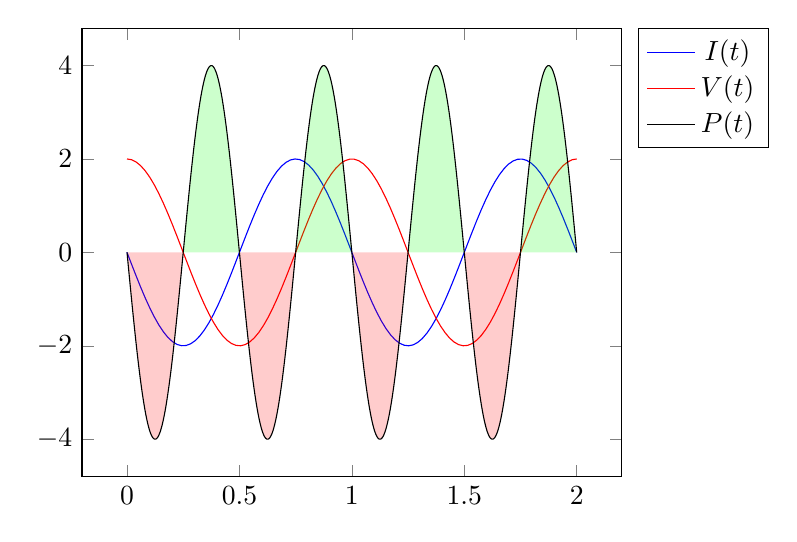
\begin{tikzpicture}
        \begin{axis}[samples=100,domain=0:2,legend pos=outer north east]
            \addplot[mark=none, blue] {-2*sin(deg(2*pi*x))}; 
            \addplot[mark=none, red] {2*cos(deg(2*pi*x))};
            \addplot[mark=none, fill=red,   domain=0:0.25, fill opacity=0.2 ] {(-4*sin(deg(4*pi*x)))};
            \addplot[mark=none, fill=green, domain=0.25:0.5, fill opacity=0.2 ] {(-4*sin(deg(4*pi*x)))};
            \addplot[mark=none, fill=red,   domain=0.5:0.75, fill opacity=0.2 ] {(-4*sin(deg(4*pi*x)))};
            \addplot[mark=none, fill=green, domain=0.75:1, fill opacity=0.2 ] {(-4*sin(deg(4*pi*x)))};
            \addplot[mark=none, fill=red,   domain=1:1.25, fill opacity=0.2 ] {(-4*sin(deg(4*pi*x)))};
            \addplot[mark=none, fill=green, domain=1.25:1.5, fill opacity=0.2 ] {(-4*sin(deg(4*pi*x)))};
            \addplot[mark=none, fill=red,   domain=1.5:1.75, fill opacity=0.2 ] {(-4*sin(deg(4*pi*x)))};
            \addplot[mark=none, fill=green, domain=1.75:2, fill opacity=0.2 ] {(-4*sin(deg(4*pi*x)))};
            \legend{$I(t)$,$V(t)$,$P(t)$}
        \end{axis}
    \end{tikzpicture}
\end{figure}
From the plot it is clear that the red and green areas are equal and opposite
and thus when integrating over a integer number of cycles the average power will
be zero.

\ex{1.28}
\begin{circuit}{fig:1.28.1}{RC Circuit with AC Voltage Source}
    (0,-2.5) node[ground](gnd){}
    (0,-2.5) to[vsourcesin,l=$V_0\cos\omega t$] (0,0)
    (0,0) to [C,l=$C$] (4,0)
    (4,-2.5) node[ground](gnd){}
    (4,0) to [R,l=$R$] (4,-2.5)
    (4,0) to[short, -o] (6.5,0) node[above]{$V_R$}
\end{circuit}
From discussions before this question, we know that 
\[P = Re(VI^*)=\frac{V_0^2R}{R^2+(\frac{1}{\omega^2C^2})}\]
And, we have the following approximation from previous discussions of highpass filters.
\[\frac{V_R}{V_0} \approx \frac{R}{R + \frac{1}{\omega C}}\]
Thus, 
\[V_R = V_0 * \frac{\omega RC}{1+\omega RC}\]
\[\frac{V_R^2}{R} =\frac{V_0^2 * \omega^2 RC^2}{(1+\omega RC)^2}\]
One way to show that all the average power delivered to the circuit above is consumed by the resistor is to find the ratio between the two.
\[\frac{\frac{V_R^2}{R}}{P} = \frac{\omega^2 R^2 C^2 + 1}{(1+\omega RC)^2}\]
Given that 
\[\omega = 2\pi f\]
we can calculate $\omega$ and plug in the numbers to find the ratio is $0.60$, which means $60\%$ of the power ends up in the resistor.

\todoex{1.29}

\ex{1.30}
$V_\out$ is simply the voltage at the output of an impedance voltage divider. We know that $Z_R = R$ and $Z_C = \frac{1}{j\omega C}$. Thus we have 
\[V_\out = \frac{Z_C}{Z_R + Z_C} V_\in = \frac{\frac{1}{j \omega C}}{R + \frac{1}{j \omega C}} V_\in = \frac{1}{1 + j \omega R C} V_\in\]
The magnitude of this expression can be found by multiplying by the complex conjugate and taking the square root.
\[\sqrt{V_\out V_\out^*} = \frac{1}{\sqrt{1 + \omega^2R^2C^2}}V_\in\]

\todoex{1.31}

\todoex{1.32}

\todoex{1.33}

\todoex{1.34}

\todoex{1.35}

\todoex{1.36}

\todoex{1.37}

\todoex{1.38}

\todoex{1.39}

\todoex{1.40}

\todoex{1.41}

\todoex{1.42}

\todoex{1.43}

\ex{1.44}
The equivalent capacitance of the oscilloscope and cable is
\[ C_o = \SI{100}{\pico\farad} + \SI{20}{\pico\farad} =  \SI{120}{\pico\farad}\]
The equivalent input impedance of the oscilloscope and the total capacitance is:
$Z_o = \left( R_o \parallel \frac{1}{j\omega C_o} \right)$
where $R_o$ is the input resistance of the scope (\SI{1}{\mega\ohm}).
In order to reduce the voltage by a factor of 10, let us create a voltage divider between the probe tip and the equivalent scope-and-cable input impedance.
\begin{circuit}{fig:1.44.1}{Basic Voltage Divider}
    (-1,0) to[open, v_<=$V_\in$] (-1,2)
    (-1,2) to[generic=$Z_{\text{probe}}$] (2,2)
    to[generic, l_=$Z_o$, *-*] (2,0)
    to[short] (-1,0)
    (2,2)  to[short, -o] (4,2)
    (2,0) to[short, -o] (4,0)
    (4,0) to[open, v_<=$V_\out$] (4,2)
\end{circuit}
In order to reduce the voltage by a factor of ten, our circuit must satisfy
\[V_{\out} = \frac{V_{\in}}{10}\]
We know that the output of a voltage divider is given by
\[V_{\out} = V_{\in}\frac{Z_{\out}}{Z_{\out} + Z_{\in}}\]
When we equate the previous two expressions, it yields
\[\frac{V_{\in}}{10} = V_{\in}\frac{Z_o}{Z_o + Z_{\text{probe}}}\]
We may cancel $V_{\in}$ from both sides of the equation and rearrange terms
\[Z_o + Z_{\text{probe}} = 10 Z_o\]
Subtract $Z_o$ from both sides to solve for the probe impedance:
\begin{align*}
    Z_{\text{probe}} &= 9 Z_o \\
    &= 9 \left( R_o \parallel \frac{1}{ j\omega C_o } \right) \\
    &= 9 R_o \parallel \frac{9}{ j\omega C_o } \\
    &= 9 R_o \parallel \frac{1}{ j\omega \left( \frac{1}{9} C_o \right) }
\end{align*}

So our ``x10 probe'' should be the parallel combination of a resistor and a capacitor.  The resistor should be 9 times greater than the input resistance of the scope ($R_o$).  The probe's capacitor should be 9 times \textit{smaller} than $C_o$ (the total capacitance of the cable and the oscilloscope).
\[R_{\text{probe}} = 9 R_o\]
\[C_{\text{probe}} = \frac{1}{9} C_o\]
\begin{circuit}{fig:1.44.2}{x10 Probe}
    (-1,0) to[open, v_<=$V_\in$, o-] (-1,2)
    (0,3) to[C, l=$C_{\text{probe}}$] (2,3)
    (0,2) to[R, l_=$R_{\text{probe}}$, *-*] (2,2)
    (0,3) to[short] (0,2)
    (2,3) to[short] (2,2)
    (0,2)  to[short, -o] (-1,2)
    (3,2) to[R, l_=$R_o$, *-*] (3,0)
    (4,0)to[C, l_=$C_o$, *-*] (4,2)
    (2,0) to[short] (-1,0)
    (2,2)  to[short, -o] (6,2)
    (2,0) to[short, -o] (6,0)
    (6,0) to[open, v_<=$V_\out$] (6,2)
\end{circuit}
Many x10 probes implement $C_{\text{probe}}$ as a variable capacitor that the user may tune to very near one ninth the cable-plus-oscilloscope capacitance.  This is sometimes referred to as ``probe compensation''.

The input impedance of this x10 probe is
\begin{align*}
    Z_{\in} &= Z_{\text{probe}} + Z_o \\
    &= 9 R_o \parallel \frac{1}{ j\omega \left( \frac{1}{9} C_o \right) } + \left( R_o \parallel \frac{1}{ j\omega C_o } \right) \\
    &= 9 \left( R_o \parallel \frac{1}{ j\omega C_o } \right) + \left( R_o \parallel \frac{1}{ j\omega C_o } \right) \\ 
    &= 10 \left( R_o \parallel \frac{1}{ j\omega C_o } \right) \\
    Z_{\in} &= \mans{ 10 Z_o }
\end{align*}
Finally, lets take a look at how the probe and the oscilloscope (working as a voltage divider) affect the output voltage as a function of the input voltage.
\begin{align*}
    \frac{V_{\out}}{V_{\in}} &= \frac{Z_o}{Z_{\in}} \\
    &= \frac{ R_o \parallel \frac{1}{ j\omega C_o } }{ 10 \left( R_o \parallel \frac{1}{ j\omega C_o } \right) } \\
    \frac{V_{\out}}{V_{\in}} &= \frac{1}{10}
\end{align*}
It is remarkable! The voltage transfer function of this circuit is \textit{precisely} $\frac{1}{10}$.  This circuit contains four passive components (two of them reactive) but \textbf{the transfer function does not depend on frequency}. Truly, the ancients were wise and knew many great things.

% Here ends Chapter 1.

%%% Local Variables:
%%% mode: latex
%%% TeX-master: "main"
%%% End:
